\documentclass[10pt]{article}
\usepackage[margin=1.55cm,top=1.45cm,bottom=1.55cm]{geometry}
\usepackage[table]{xcolor}
\usepackage{tikz}
\usetikzlibrary{arrows.meta,positioning,shapes.geometric,fit}
\usepackage[most]{tcolorbox}
\usepackage{tabularx,booktabs,array,multicol}
\usepackage{enumitem}
\usepackage{fancyhdr}
\usepackage{hyperref}
\usepackage{microtype}
\usepackage[T1]{fontenc}
\usepackage{lmodern}

\definecolor{Midnight}{HTML}{0B132B}
\definecolor{Navy}{HTML}{14213D}
\definecolor{Teal}{HTML}{00A6A6}
\definecolor{Mint}{HTML}{E6F7F5}
\definecolor{Coral}{HTML}{FF6B5E}
\definecolor{Amber}{HTML}{F4B942}
\definecolor{Cloud}{HTML}{F4F7FA}
\definecolor{Ink}{HTML}{1E293B}
\definecolor{Slate}{HTML}{64748B}
\definecolor{Line}{HTML}{D9E2EC}

\hypersetup{colorlinks=true,linkcolor=Teal,urlcolor=Teal,pdftitle={SchemaForge Hackathon Brief},pdfauthor={SchemaForge Team}}
\renewcommand{\familydefault}{\sfdefault}
\setlength{\parindent}{0pt}
\setlength{\parskip}{4pt}
\setlist[itemize]{leftmargin=1.25em,itemsep=2pt,topsep=3pt}
\pagestyle{fancy}
\fancyhf{}
\fancyhead[L]{\textcolor{Slate}{\small SchemaForge \textbullet\ Agents That Act}}
\fancyhead[R]{\textcolor{Slate}{\small September 2026}}
\fancyfoot[C]{\textcolor{Slate}{\small \thepage}}
\renewcommand{\headrulewidth}{0pt}

\newtcolorbox{card}[1]{enhanced,breakable,colback=Cloud,colframe=Line,boxrule=0.6pt,arc=3mm,left=3mm,right=3mm,top=2.5mm,bottom=2.5mm,title=#1,coltitle=Midnight,fonttitle=\bfseries,attach boxed title to top left={xshift=2mm,yshift=-1.5mm},boxed title style={colback=white,colframe=Line,boxrule=0.5pt,arc=2mm}}
\newtcolorbox{accentcard}[1]{enhanced,breakable,colback=Mint,colframe=Teal,boxrule=0.8pt,arc=3mm,left=3mm,right=3mm,top=2.5mm,bottom=2.5mm,title=#1,coltitle=Midnight,fonttitle=\bfseries}
\newcommand{\pill}[2]{\tikz[baseline=-0.6ex]\node[rounded corners=5pt,fill=#1,inner xsep=6pt,inner ysep=2.5pt,text=white,font=\scriptsize\bfseries]{#2};}
\newcommand{\metric}[2]{\begin{minipage}[t]{0.23\linewidth}\centering{\Large\bfseries\textcolor{Teal}{#1}}\\[-1mm]{\scriptsize\textcolor{Slate}{#2}}\end{minipage}}

\begin{document}

% ── Cover ───────────────────────────────────────────────────────
\thispagestyle{empty}
\pagecolor{Midnight}\color{white}
\vspace*{1.2cm}
{\small\bfseries\textcolor{Teal}{TRUEFOUNDRY \(\times\) POLARIS \textbullet\ AGENTS THAT ACT}}\\[8mm]
{\fontsize{42}{46}\selectfont\bfseries SchemaForge}\\[4mm]
{\LARGE An agent that rehearses database migrations,\\proves what happened, and knows when to stop.}

\vspace{10mm}
\begin{tcolorbox}[colback=Navy,colframe=Teal,boxrule=0.9pt,arc=4mm,left=5mm,right=5mm,top=5mm,bottom=5mm]
\color{white}\large
A human states a PostgreSQL change in plain language. SchemaForge inspects the live target, maps dependencies, executes generated SQL inside a rollback-only shadow sandbox, verifies explicit assertions and rollback equivalence, then freezes before production. Applying requires both a signed exact-action token and TrueForge's visible Allow/Deny checkpoint.
\end{tcolorbox}

\vfill
\begin{center}
\metric{6}{typed MCP tools}\hfill
\metric{2}{isolated services}\hfill
\metric{2}{human gates}\hfill
\metric{0}{blind prod writes}
\end{center}
\vfill

\begin{minipage}{0.66\linewidth}
\textcolor{white}{\bfseries Repository}\\
\href{https://github.com/harshaxyZ/schemaforge}{github.com/harshaxyZ/schemaforge}
\end{minipage}
\begin{minipage}{0.32\linewidth}\raggedleft
\pill{Teal}{EVIDENCE FIRST}\quad\pill{Coral}{HUMAN GATED}
\end{minipage}
\newpage
\nopagecolor\color{Ink}

% ── Challenge fit ───────────────────────────────────────────────
\section*{Built for the challenge, not around it}
The official challenge asks for an agent that reaches a real system, runs generated code safely, and pauses before irreversible action. SchemaForge is the featured ``Migration Rehearsal Agent'' pattern made concrete.

\begin{tabularx}{\textwidth}{>{\bfseries\color{Midnight}}p{0.22\textwidth} X >{\centering\arraybackslash}p{0.13\textwidth}}
\toprule
Requirement & Verifiable implementation & Status \\
\midrule
Runs on TrueForge & Current agent spec, focused instructions, remote Streamable HTTP MCP connectors, and sandbox enabled. & \pill{Teal}{YES} \\
Real system & PostgreSQL 16 target reached with a database-enforced read-only role. & \pill{Teal}{YES} \\
Safe generated code & Migration SQL runs on a separate shadow database in one serialized transaction, then always rolls back. & \pill{Teal}{YES} \\
Human checkpoint & MCP \texttt{destructiveHint}, explicit TrueForge tool gate, signed five-minute token, and human \texttt{--confirm}. & \pill{Teal}{YES} \\
Secrets protected & Core has no write credential or signing key; role env files and runtime state are ignored by Git. & \pill{Teal}{YES} \\
Explainable build & Deterministic rules and evidence are implemented in small TypeScript modules; AI use is disclosed. & \pill{Teal}{YES} \\
\bottomrule
\end{tabularx}

\vspace{4mm}
\begin{multicols}{2}
\begin{accentcard}{Why this matters}
Database migrations combine model uncertainty with high-blast-radius actions. A plausible SQL answer is not proof. SchemaForge converts the risky leap from ``looks right'' to ``run it'' into a measured control loop with a deliberate human boundary.
\end{accentcard}

\begin{card}{Two demo outcomes}
\textbf{Knows when to stop:} adding \texttt{NOT NULL UNIQUE} to seeded emails exposes 14 NULLs and a duplicate group; rehearsal fails and production remains untouched.

\textbf{Acts when proven safe:} an additive phone column rehearses, verifies, rolls back cleanly, pauses twice, and then commits with drift and postcondition checks.
\end{card}
\end{multicols}

\section*{System architecture}
\begin{center}
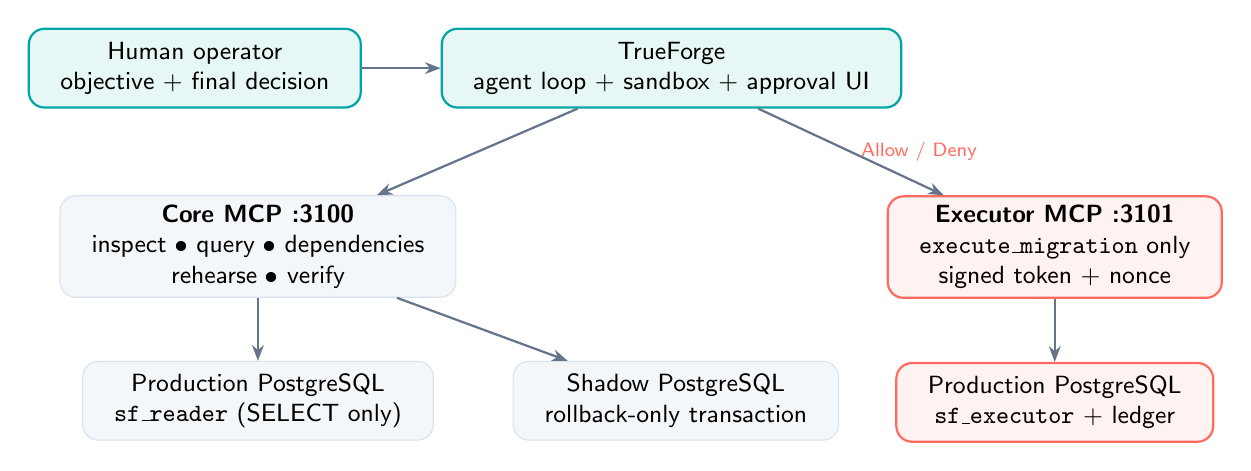
\begin{tikzpicture}[
  node distance=8mm and 10mm,
  box/.style={draw=Line,fill=Cloud,rounded corners=2mm,minimum height=10mm,align=center,font=\small,inner xsep=4mm},
  strong/.style={box,draw=Teal,fill=Mint,line width=0.8pt},
  risk/.style={box,draw=Coral,fill=Coral!8,line width=0.8pt},
  arrow/.style={-{Stealth[length=2mm]},line width=0.8pt,draw=Slate}
]
\node[strong] (human) {Human operator\\objective + final decision};
\node[strong,right=of human] (tf) {TrueForge\\agent loop + sandbox + approval UI};
\node[box,below left=11mm and -2mm of tf] (core) {\textbf{Core MCP :3100}\\inspect \textbullet\ query \textbullet\ dependencies\\rehearse \textbullet\ verify};
\node[risk,below right=11mm and -2mm of tf] (exec) {\textbf{Executor MCP :3101}\\\texttt{execute\_migration} only\\signed token + nonce};
\node[box,below=of core] (prodro) {Production PostgreSQL\\\texttt{sf\_reader} (SELECT only)};
\node[box,right=of prodro] (shadow) {Shadow PostgreSQL\\rollback-only transaction};
\node[risk,below=of exec] (prodwr) {Production PostgreSQL\\\texttt{sf\_executor} + ledger};
\draw[arrow] (human) -- (tf);
\draw[arrow] (tf) -- (core);
\draw[arrow] (tf) -- node[right,font=\scriptsize,text=Coral]{Allow / Deny} (exec);
\draw[arrow] (core) -- (prodro);
\draw[arrow] (core) -- (shadow);
\draw[arrow] (exec) -- (prodwr);
\end{tikzpicture}
\end{center}

\newpage
% ── Safety mechanics ────────────────────────────────────────────
\section*{The action boundary is enforced in code}

\begin{multicols}{2}
\begin{card}{Before rehearsal}
\begin{itemize}
  \item Stable schema fingerprint excludes row-count estimates and internal ledger state.
  \item Dependency catalog covers foreign keys, views, materialized views, functions, triggers, indexes, policies, and sequences.
  \item Fail-closed SQL allowlist rejects Tier-3, DML, internal-ledger access, ambiguous escapes, unknown, mixed, and non-transactional plans.
\end{itemize}
\end{card}

\begin{card}{Inside the shadow sandbox}
\begin{itemize}
  \item One physical PostgreSQL connection owns \texttt{BEGIN}, SQL, assertions, rollback test, and final \texttt{ROLLBACK}.
  \item Explicit assertions evaluate values; successful execution alone never passes.
  \item Returns observed timing, lock snapshot, notices, exact row counts, and three fingerprints.
\end{itemize}
\end{card}

\begin{card}{At human approval}
\begin{itemize}
  \item HMAC covers exact SQL and assertion-set hashes, baseline/post fingerprints, rehearsal ID, action, target, UUID nonce, and expiry.
  \item The model never receives the signing secret and cannot mint a token.
  \item TrueForge independently gates the destructive-annotated tool call.
\end{itemize}
\end{card}

\begin{card}{During production execution}
\begin{itemize}
  \item Nonce is atomically claimed, preventing replay and ambiguous retries.
  \item Advisory lock serializes SchemaForge applies; lock and statement timeouts cap impact.
  \item Drift check, DDL, approved assertions, post-fingerprint check, and success-ledger update form one transaction.
\end{itemize}
\end{card}
\end{multicols}

\begin{accentcard}{Defense in depth}
\centering
\pill{Navy}{READ-ONLY ROLE}\quad
\pill{Navy}{SHADOW DB}\quad
\pill{Navy}{SQL POLICY}\quad
\pill{Navy}{SIGNED TOKEN}\quad
\pill{Navy}{NONCE LEDGER}\quad
\pill{Navy}{TRUEFORGE GATE}
\end{accentcard}

\section*{Evidence-driven workflow}
\begin{tabularx}{\textwidth}{>{\centering\arraybackslash\bfseries\color{Teal}}p{0.045\textwidth} >{\bfseries}p{0.22\textwidth} X}
\rowcolor{Midnight} \textcolor{white}{\#} & \textcolor{white}{Stage} & \textcolor{white}{Observable output} \\
\rowcolor{Cloud} 1 & Parse intent & Objective, affected objects, explicit success condition \\
2 & Inspect & Catalog, PostgreSQL metadata, baseline SHA-256 \\
\rowcolor{Cloud} 3 & Dependencies & Exact blast-radius categories and object definitions \\
4 & Synthesize & Byte-stable forward SQL, honest rollback, transaction class \\
\rowcolor{Cloud} 5 & Rehearse & Timings, locks, notices, row deltas, post fingerprint \\
6 & Verify & Named machine assertions plus rollback fingerprint equality \\
\rowcolor{Cloud} 7 & Assess & Deterministic \texttt{APPLY / REVIEW / DO\_NOT\_APPLY} recommendation \\
8 & Freeze & Complete decision packet; no production call in the same turn \\
\rowcolor{Cloud} 9 & Execute & New human message, signed token, TrueForge Allow, ledgered result \\
\end{tabularx}

\vspace{3mm}
\textcolor{Slate}{\small Measurement discipline: tool-returned values are labeled \textbf{[OBSERVED]}; catalog statistics and reasoned projections are \textbf{[ESTIMATED]}. A lock snapshot is never presented as an exact lock duration.}

\newpage
% ── Demo and operation ──────────────────────────────────────────
\section*{Judge demo: failure first, then safe action}

\begin{card}{01 \quad Prove that stopping is a feature}
\textbf{Prompt:} ``Make \texttt{users.email} NOT NULL and UNIQUE. Prove it is safe before applying anything.''

The shared deterministic seed contains 500 users, exactly 14 NULL emails, and three rows sharing \texttt{duplicate@example.com}. Inspection and data queries surface the violations. Naive DDL fails in the shadow transaction, the tool returns \texttt{DO\_NOT\_APPLY}, and SchemaForge freezes without calling the executor.
\end{card}

\begin{card}{02 \quad Demonstrate controlled agency}
\textbf{Prompt:} ``Add an optional \texttt{phone VARCHAR(32)} column. Rehearse it, verify rollback, and prepare a decision packet.''

The agent runs forward SQL, evaluates a catalog assertion, captures the post fingerprint, runs rollback SQL, proves baseline restoration, and presents the packet. The operator signs the exact SQL outside the agent. A new turn calls the destructive tool; TrueForge pauses. On Allow, the executor checks drift and postconditions before commit. Reusing the token proves replay rejection.
\end{card}

\section*{Fast local launch}
\begin{tcolorbox}[colback=Midnight,colframe=Midnight,arc=3mm,left=4mm,right=4mm,top=3mm,bottom=3mm]
\ttfamily\small\color{white}
\$ npm run setup\qquad\$ npm run build\\
\$ docker compose up -d\\
\$ npm run start:core\qquad\# terminal 1\\
\$ npm run start:executor\quad\# terminal 2\\
\$ npx @truefoundry/trueforge@0.2.1
\end{tcolorbox}

\begin{multicols}{2}
\begin{accentcard}{What judges can inspect}
\begin{itemize}
  \item Six typed MCP tools with correct annotations
  \item Separate core/executor credentials and ports
  \item SQL policy and HMAC verifier
  \item Durable production nonce/outcome ledger
  \item Deterministic edge-case data
  \item Focused TrueForge agent instructions
\end{itemize}
\end{accentcard}

\begin{card}{Deliberate limits}
SchemaForge's atomic executor refuses all DML, concurrent-index and other non-transactional DDL rather than pretending it can roll them back. It also refuses role administration, database/schema/table deletion, procedural escape hatches, internal-ledger access, and SQL outside its canonical fingerprint model. Safe inability is part of the product.
\end{card}
\end{multicols}

\section*{Build story}
The first prototype had the right narrative but unsafe mechanics: stdio-only transport, mismatched environment names, pool-level pseudo-transactions, a caller-authored ``token,'' persistent shadow state, and verification-by-query-success. The v2.1 build replaced each promise with an enforceable boundary and rewrote the public documentation to describe only what the code does.

\vfill
\begin{tabularx}{\textwidth}{X >{\raggedleft\arraybackslash}X}
\textbf{Team principle} & \textbf{Model proposes. Tools measure. Policy constrains. Human decides.}\\
\textcolor{Slate}{AI assistance: Kiro IDE with Claude Opus 5; architecture remains team-owned and explainable.} & \href{https://github.com/harshaxyZ/schemaforge}{View source}\\
\end{tabularx}

\vspace{2mm}
{\scriptsize\textcolor{Slate}{Sources: official HackCulture event brief and rules; TrueForge repository and documentation for agent specs, MCP connectors, sandboxing, and human checkpoints. Descriptions are paraphrased for licensing compliance.}}

\end{document}
